\apendice{Especificación de diseño}

\section{Introducción}

En este apartado se describe el diseño del sistema desarrollado, abordando su organización interna, la estructura de los datos gestionados y el comportamiento de los distintos módulos que componen los addons implementados para Blender.

El sistema está constituido por dos addons independientes pero complementarios: un addon de recopilación de datos, responsable de la detección y registro de eventos durante la interacción del usuario con el entorno de modelado, y un addon de análisis, encargado de procesar los datos generados y presentar métricas de forma visual. Ambos componentes se comunican mediante archivos intermedios en formato CSV, lo que permite mantener una arquitectura desacoplada, flexible y fácilmente extensible.

El diseño del sistema se ha realizado siguiendo principios clásicos de ingeniería del software, como la modularidad, la separación de responsabilidades, el bajo acoplamiento y la alta cohesión. Estos criterios permiten mejorar la mantenibilidad del sistema, facilitar su evolución futura y asegurar la coherencia entre los requisitos definidos, la implementación realizada y los resultados obtenidos.

Con el fin de estructurar la descripción del sistema de manera clara y completa, este apartado se organiza en tres niveles: diseño de datos, diseño arquitectónico y diseño procedimental.

\section{Diseño de datos}

El sistema utiliza archivos CSV como mecanismo principal de persistencia de datos. En estos archivos se almacenan los eventos capturados durante la interacción del usuario con Blender, permitiendo su posterior procesamiento por el addon de análisis.

La estructura de los datos se ha diseñado siguiendo un modelo semiestructurado orientado a eventos, en el que cada registro representa una acción significativa realizada por el usuario en el entorno de modelado. Este enfoque permite reconstruir la secuencia de acciones y analizar el comportamiento del usuario de forma temporal.

Cada fila del archivo corresponde a un evento detectado por el sistema. La información almacenada combina datos temporales, identificativos y geométricos, proporcionando una visión completa del estado del sistema en el momento de la interacción.

La Figura~\ref{fig:diseno_datos} muestra la estructura lógica de los datos gestionados por el sistema.

\begin{figure}[H]
    \centering
    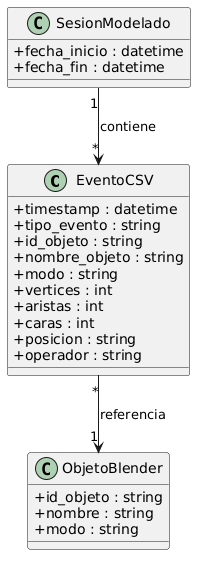
\includegraphics[height=0.85\textheight, keepaspectratio]{diagramas/diseno_datos.png}
    \caption{Estructura lógica de los datos registrados por el sistema.}
    \label{fig:diseno_datos}
\end{figure}

De forma general, cada evento incluye los siguientes campos:

\begin{itemize}
    \item \textbf{timestamp}: marca temporal exacta del evento.
    \item \textbf{tipo\_evento}: tipo de acción registrada.
    \item \textbf{id\_objeto}: identificador único del objeto afectado.
    \item \textbf{nombre\_objeto}: nombre asignado al objeto en la escena.
    \item \textbf{modo}: modo de trabajo activo en el momento del evento.
    \item \textbf{propiedades}: conjunto de atributos geométricos o contextuales relevantes.
\end{itemize}

La elección del formato CSV responde a criterios de simplicidad, interoperabilidad y eficiencia, facilitando tanto el almacenamiento como la inspección manual y el procesamiento externo de los datos.

\section{Diseño arquitectónico}

La arquitectura del sistema se basa en un modelo modular orientado a la separación de responsabilidades. Este diseño sigue los principios de bajo acoplamiento y alta cohesión, permitiendo la evolución independiente de los distintos módulos y facilitando su mantenimiento.

La Figura~\ref{fig:diseno_arquitectura} presenta la arquitectura general del sistema en formato vertical, donde se muestra el flujo de datos desde la interacción del usuario hasta la visualización de métricas.

\begin{figure}[H]
    \centering
    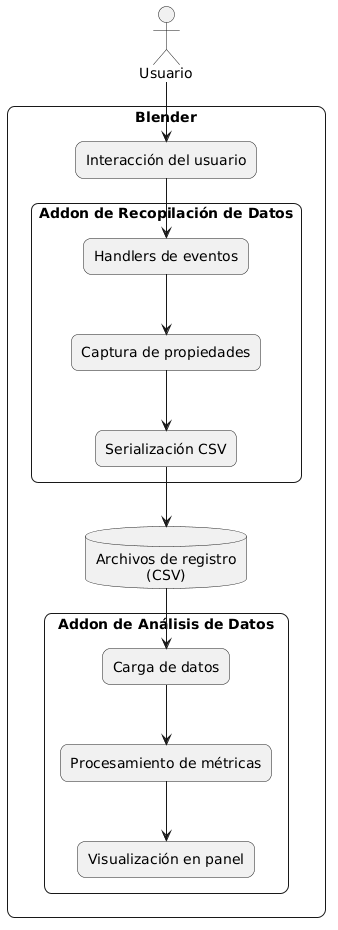
\includegraphics[height=0.85\textheight, keepaspectratio]{diagramas/diseno_arquitectura_vertical.png}
    \caption{Arquitectura vertical del sistema.}
    \label{fig:diseno_arquitectura}
\end{figure}

Asimismo, la Figura~\ref{fig:diseno_componentes} representa el sistema desde el punto de vista de componentes software, mostrando las dependencias y relaciones entre los distintos módulos.

\begin{figure}[H]
    \centering
    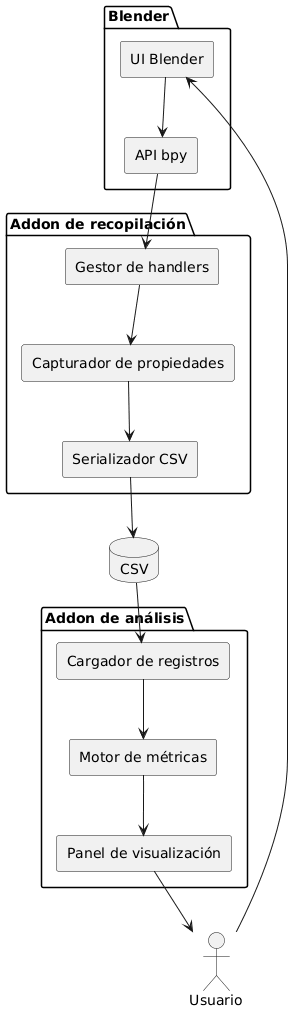
\includegraphics[height=0.85\textheight, keepaspectratio]{diagramas/diseno_componentes.png}
    \caption{Diagrama de componentes del sistema.}
    \label{fig:diseno_componentes}
\end{figure}

A nivel funcional, la arquitectura puede descomponerse en los siguientes bloques:

\begin{itemize}
    \item Interacción del usuario en el entorno de Blender.
    \item Detección de eventos mediante handlers.
    \item Captura y estructuración de datos.
    \item Persistencia en archivos CSV.
    \item Carga y procesamiento de datos.
    \item Visualización de métricas en la interfaz.
\end{itemize}

Este enfoque arquitectónico permite desacoplar la captura del análisis, facilitando la reutilización de datos y la extensión futura del sistema.

\section{Diseño procedimental}

El diseño procedimental describe la secuencia de operaciones que ejecuta el sistema en respuesta a las acciones del usuario.

La Figura~\ref{fig:diseno_procedimental} muestra el flujo completo del sistema, desde la interacción inicial hasta la generación de resultados.

\begin{figure}[H]
    \centering
    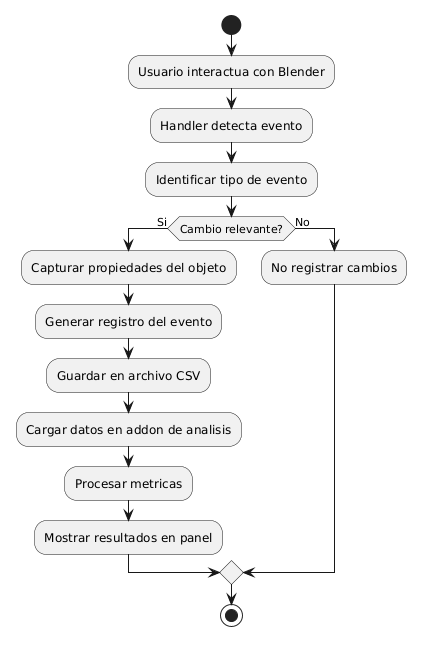
\includegraphics[width=0.65\textwidth]{diagramas/diseno_procedimental.png}
    \caption{Flujo procedimental del sistema.}
    \label{fig:diseno_procedimental}
\end{figure}

Por su parte, la Figura~\ref{fig:diseno_secuencia} describe la interacción temporal entre los distintos componentes del sistema.

\begin{figure}[H]
    \centering
    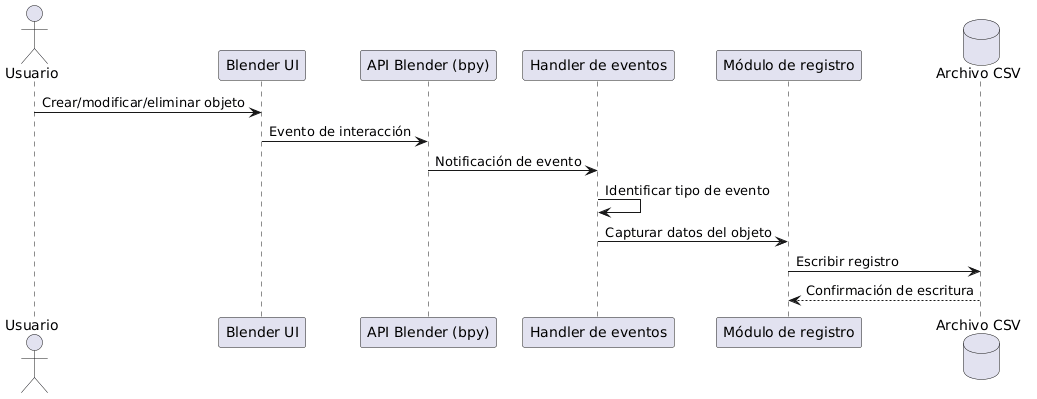
\includegraphics[width=0.85\textwidth]{diagramas/secuencia.png}
    \caption{Diagrama de secuencia del sistema.}
    \label{fig:diseno_secuencia}
\end{figure}

El flujo general de ejecución es el siguiente:

\begin{enumerate}
    \item El usuario realiza una acción en Blender.
    \item El sistema detecta el evento mediante los handlers registrados.
    \item Se identifican el tipo de acción y el objeto afectado.
    \item Se capturan las propiedades relevantes.
    \item Se genera un registro estructurado del evento.
    \item El registro se almacena en el archivo CSV correspondiente.
    \item El addon de análisis procesa los datos y genera métricas.
    \item Los resultados se presentan en la interfaz de usuario.
\end{enumerate}

El sistema optimiza el rendimiento evitando el registro de información redundante, almacenando únicamente cambios significativos en el estado de los objetos. Este enfoque orientado a eventos se adapta de forma natural al modelo de ejecución de Blender, permitiendo una integración eficiente con su API.

\section{Decisiones de diseño relevantes}

Durante el desarrollo del sistema se han adoptado varias decisiones clave que condicionan su comportamiento y estructura:

\begin{itemize}
    \item \textbf{Separación en dos addons}: permite desacoplar la captura de datos del análisis, facilitando la mantenibilidad y evolución del sistema.
    \item \textbf{Uso de CSV como formato de persistencia}: proporciona una solución ligera, interoperable y fácilmente depurable.
    \item \textbf{Captura basada en handlers}: permite detectar automáticamente eventos en Blender sin intervención directa del usuario.
    \item \textbf{Procesamiento diferido de métricas}: evita sobrecargar el sistema durante la captura de datos.
    \item \textbf{Registro selectivo de cambios}: reduce el volumen de datos y mejora la eficiencia.
\end{itemize}

Estas decisiones garantizan un sistema robusto, eficiente y alineado con los requisitos definidos.

Por último, la Figura~\ref{fig:arquitectura} presenta una visión global del sistema, integrando los dos addons desarrollados y mostrando el flujo completo de información entre ellos.

\begin{figure}[H]
    \centering
    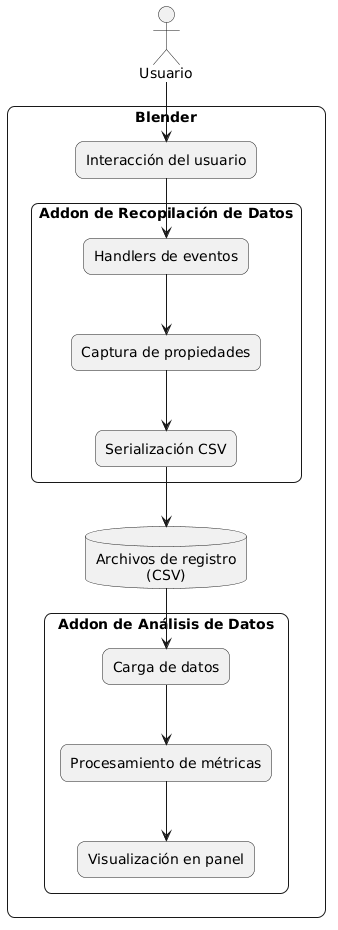
\includegraphics[height=0.85\textheight, keepaspectratio]{diagramas/diseno_arquitectura_vertical.png}
    \caption{Arquitectura general del sistema basada en dos addons independientes.}
    \label{fig:arquitectura}
\end{figure}